%! Author = Len Washington III
%! Date = 9/19/2023

% Preamble
\documentclass[12pt]{report}

% Packages
\usepackage[10]{cs430lecture}

% Document
\begin{document}

%<*Lecture-Activity-10>
\newcommand{\bsttree}{\tikzset{every tree node/.style={minimum width=2em,draw,circle},
         blank/.style={draw=none},
         edge from parent/.style=
         {draw,edge from parent path={(\tikzparentnode) -- (\tikzchildnode)}},
         level distance=1cm}
			\begin{tikzpicture}
			\Tree
			[.$15$
				[.$6$
					[.$3$
						[.$2$ ]
						[.$4$ ]
					]
					[.$7$
						[.$13$
							[.$9$ ]
						]
					]
				]
				[.$18$
					[.$17$ ]
					[.$20$ ]
			]]
			\end{tikzpicture}}
\section{Opening Questions}\label{sec:opening-questions-10}
\begin{enumerate}[label=\arabic*.]
    \item In your own words explain how you insert a new key in a binary search tree.
	\item Give an example of a series of 5 keys inserted one at a time into a binary search tree that will yield a tree of height 5.
	\item If we do a left rotate on node $X$ below, explain which left and/or right child links need to be changed.\\
\tikzset{every tree node/.style={minimum width=2em},
         blank/.style={draw=none},
         edge from parent/.style=
         {draw,edge from parent path={(\tikzparentnode) -- (\tikzchildnode)}},
         level distance=1cm}
	\begin{tikzpicture}
		\Tree
		[.$X$
			[.$a$ ]
			[.$Y$
				[.$b$ ]
				[.$c$ ]
		]]
		\end{tikzpicture}
\end{enumerate}

\section{Tree depth vs Tree Height}\label{sec:tree-depth-vs-tree-height}
The length of the path from the root $r$ to a node $x$ is the depth of $x$ in $T$. The height of a node in a tree is the number of edges on the longest simple downward path from the node to a leaf, and the height of a tree is the height of its root. The height of a tree is also equal to the largest depth of any node in the tree.
\begin{figure}[H]
	\centering
	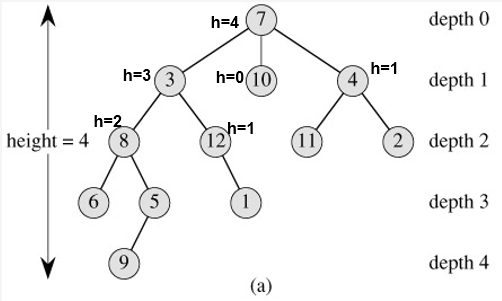
\includegraphics[width=\textwidth]{10.1}
	\caption{Height vs Depth of a Tree}
	\label{fig:tree-height-depth}
\end{figure}

\section{BST Operations}\label{sec:bst-operations}
\begin{enumerate}[label=\arabic*)]
    \item Write pseudocode for BST Successor (or Predecessor). Demonstrate on the below tree from node 15 and then node 13.\\\bsttree
	\item Write pseudocode for BST Insert. Demonstrate on the below tree to insert 5 and then 19.\\\bsttree
	\item What are the three possible cases when deleting a node from a BST?
	\item Write pseudocode for BST Delete (assume you already have a pointer to the node)
\end{enumerate}

\section{BST Rotations}\label{sec:bst-rotations}
Local operation in a search tree that maintains the BST property and possibly alters the height of the BST.\\

$x$ and $y$ are nodes; $a$, $b$, $c$ are sub trees
\tikzset{every tree node/.style={minimum width=2em},
         blank/.style={draw=none},
         edge from parent/.style=
         {draw,edge from parent path={(\tikzparentnode) -- (\tikzchildnode)}},
         level distance=1cm}
\begin{tikzpicture}
	\begin{scope}
		\begin{tikzpicture}
		\Tree
		[.$x$
			[.$a$ (l1) ]
			[.$y$
				[.$b$ ]
				[.$c$ ]
		]]
		\end{tikzpicture}
	\end{scope}
	\begin{scope}[xshift=40cm]
		\begin{tikzpicture}
		\Tree
		[.$y$
			[.$x$
				[.$a$ ]
				[.$b$ ]
			]
			[.$c$ ]
		]
		\end{tikzpicture}
	\end{scope}
\end{tikzpicture}		% TODO: Fix this

\begin{enumerate}[label=\arabic*.,start=5]
    \item Write pseudocode for LeftRotate (or RightRotate). What is the worst case runtime?
\end{enumerate}

%</Lecture-Activity-10>

\end{document}